\begin{itemize}
	\item Falls $\rho_V\neq 0$ wird die Vakuumdichte ab einem gewissen Zeitpunkt dominant!
	\item dimensionslose Dichteparameter:
		\begin{equation*}
			\Omega_m :=\frac{\rho_{m,0}}{\rho_c},\quad\Omega_r :=\frac{\rho_{r,0}}{\rho_c},\quad\Omega_\Lambda :=\frac{\Lambda}{3H_0^2}
		\end{equation*}
		mit der kritischen Dichte $\rho_c=\frac{3H_0^2}{8\pi G}$
	\item heutige Werte:
		\begin{itemize}[label={}]
			\item Staub:
				\begin{itemize}[label={}]
					\item Galaxien (inklusive ihrer dunklen Halos): $\Omega_m\gtrsim\num{0.02}$
					\item Galaxienhaufen $\Omega_m\gtrsim\num{0.1}$
					\item Kosmologie $\Omega_m\sim\num{0.3}$
				\end{itemize}
			\item Strahlung: Photonen der CMB + Neutrinos aus dem frühen Universum $\Omega_r\sim\num{4.2e-5}\cdot \underset{\underset{\approx\num{0.72}}{\rotatebox{90}{=}}}{h^{-2}}$
			\item Vakuum: $\Omega_\Lambda\sim\num{0.7}$
		\end{itemize}
	\item Da $H(t)=\frac{\dot{a}(t)}{a(t)}$ und $\rho=\rho_{m,0}\cdot a^{-3}(t)+\rho_{r,0}\cdot a^{-4}(t)$
		\begin{itemize}
			\item $H^2(t)=H_0^2\left[a^{-4}(t)\cdot\Omega_r+a^{-3}(t)\Omega_m-a^{-2}(t)\frac{K\cdot c^2}{H_0^2}+\Omega_\Lambda\right]$
		\end{itemize}
	\item Für $t=t_0$ (heute) mit $a(t_0)=1$ ergibt sich (mit $H(t_0)=H_0$):
		\begin{equation*}
			K=\left(\frac{H_0}{c}\right)^2\cdot\big(\Omega_m+\underset{\underset{\text{(für $t=t_0$)}}{\text{vernachlässigbar}}}{\underbrace{\Omega_r}}+\Omega_\Lambda -1\big)
		\end{equation*}
		und schließlich:
		\begin{equation*}
			\left(\frac{\dot{a}}{a}\right)^2=H^2(t)=H_0^2\left(a^{-4}(t)\cdot\Omega_r+a^{-3}(t)\cdot\Omega_m+a^{-2}(t)\cdot (1-\Omega_m-\Omega_\Lambda)+\Omega_\Lambda\right)\qquad (\ast)
		\end{equation*}
	\item \textbf{Diskussion}:
		\begin{itemize}[label={\textbullet}]
			\item Für $a<<1$ dominiert der erste (strahlungsdominiertes Universum)
			\item Für etwasa größeres $a$ dominiert der zweite Term, der Staub- (oder Materie)-Term
			\item Für $K\neq 0$ wird für größere $a$ der dritte Term dominieren
			\item Falls $\Lambda\neq 0$, dominiert die Kosmologische Konstante für $a>>1$
		\end{itemize}
	\item DGL $(\ast)$ ist nicht analytisch lösbar
	\item Einige wichtige Spezialfälle:
		\begin{itemize}
			\item[Einstein (1917)] $K>0,\Lambda\sim a^{-2}$ statisch
			\item[de Sitter (1917)] $K=\sigma,\Lambda>\sigma$
			\item[Lena\^itre (1950)] $K>0,\Lambda>a^{-2}$
			\item[Friedmann (1922)] $K\geqleq\sigma,\Lambda =\sigma$
				\begin{figure}[H]
					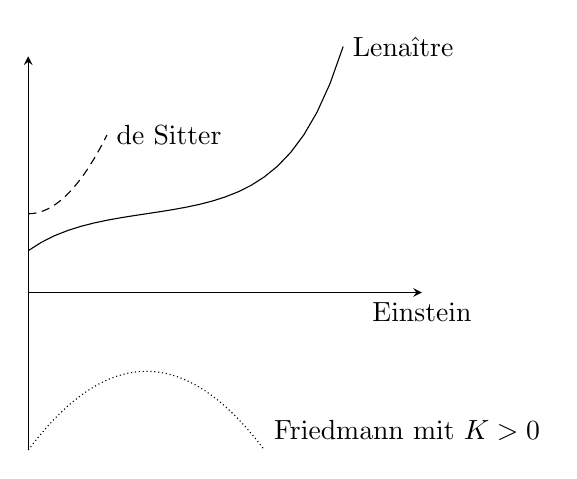
\begin{tikzpicture}[>=stealth]
						\draw[->] (0,-2)--(0,3);
						\draw[->] (0,0)--(5,0)node[below]{Einstein};
						\draw[densely dashed, domain=0:1] plot(\x,{(\x)^2+1})node[right]{de Sitter};
						\draw[domain=-1.5:2.5] plot(\x+1.5,{0.1*sinh(1.5*\x)+1})node[right]{Lena\^itre};
						\draw[densely dotted, domain=-1.5:1.5] plot(\x+1.5,{-(\x)^2/2.25-1})node[above right]{Friedmann mit $K>0$};
					\end{tikzpicture}
				\end{figure}
				\noindent$\Rightarrow$ viele Möglichkeiten\\
				Klassifikation in Abhängigkeit von $\Omega_\Lambda$ und $\Omega_m$
				\begin{figure}[H]
					\begin{tikzpicture}[>=stealth]
						\draw[domain=0:4] plot({\x},{exp(\x/4)/2.7345/2});
						\fill[pattern=north east lines, pattern color=green, domain=0:4] (0,-2.2)--(0,0)--plot({\x},{exp(\x/4)/2.7345/2})--(4,-2.2)--(0,-2.2);
						\draw[->] (0,-2.2)--(0,2.2)node[above left]{$\Omega_\Lambda$};
						\draw[->] (0,0)--(4,0)node[below right]{$\Omega_m$};
						\node at (0.8,2.5){$a>a_0\forall t$};
						\draw (0,1)--(1,2.2);
						\fill[pattern=north west lines, pattern color=green] (0,1)--(1,2.2)--(0,2.2)--cycle;
						\draw (0,1)--(4,-2);
						\node[fill=white,right] at (0.5,-2){offen ($K<0$)};
						\node[fill=white,right] at (3.5,-1){geschlossen ($K>0$)};
						\node[] at (2.5,-0.5){\textbf{Kollaps}};
						\node[] at (2.5,1){\textbf{Expansion}};
					\end{tikzpicture}
				\end{figure}
		\end{itemize}
	\item Im Gegensatz zur Newtonschen Kosmologie sind offen \& Expansion bzw. geschlossen \& Kollaps nicht mehr identisch\\
		Für $\Omega_\Lambda < 1$ gilt immer $H^2>0\forall a\leq 1$
		\begin{itemize}
			\item $\exists$ ein Zeitpunkt in der Vergangenheit mit $a(t)\to 0$
			\item "`Größe"' des Universums verschwindend klein
			\item \textbf{Urknall}
		\end{itemize}
		\textbf{\underline{N.B}}\\
		Die Möglichkeit $\Omega_\Lambda >1$ ohne Urknall kann inzwischen durch Beobachtungen ausgeschlossen werden
	\item \textbf{Abbremsparameter}
		\begin{equation*}
			q_0:=-\frac{\ddot{a}\cdot a}{a^2}\big|_{t=t_0}\underset{(F1)(F2)}{=}\frac{1}{2}\Omega_m-\Omega_\Lambda
		\end{equation*}
		\begin{itemize}[label={\textbullet}]
			\item Für den Fall $\Omega_\Lambda=0$ ist $q_0>0,\ddot{a}<0$, d.h. die Expansion wird abgebremst
			\item Falls $\Omega_\Lambda$ genügend groß ist $\Rightarrow q_0<0\Rightarrow \ddot{a}>0$
				\begin{itemize}[label={$\Rightarrow$}]
					\item \textbf{beschleunigte Expansion} (wg. negativem Druck der Vakuumenergie)
				\end{itemize}
			\item Beobachtungen deuten darauf hin, dass dies tatsächlich seit einigen $\si{Ga}$ passiert
		\end{itemize}
	\item \textbf{Weltalter}
		\begin{align*}
			dt&=\frac{da}{\left(\frac{da}{dt}\right)}=\frac{da}{a\cdot H}\\
			\Rightarrow t(a)&=\frac{1}{H_0}\int\limits_0^ada'\left[(a')^{-2}\cdot\Omega_r+(a')^{-1}\Omega_m+\left(1-\Omega_m-\Omega_\Lambda\right)\cdot(a')^{-2}+(a')^2\Omega_\Lambda\right]^{-\frac{1}{2}}
		\end{align*}
		\begin{align*}
			t_0&=t(1)\\
			&=\frac{1}{H_0}\int\limits_0^1da'\left[(a')^{-2}\cdot\Omega_r+(a')^{-1}\Omega_m+\left(1-\Omega_m-\Omega_\Lambda\right)\cdot(a')^{-2}+(a')^2\Omega_\Lambda\right]^{-\frac{1}{2}}
		\end{align*}
	\item Zwei wichtige Familien von Modellen:
		\begin{enumerate}[label={$(\roman*)$}]
			\item $\Omega_\Lambda = 0$ (da keine "`vernünftige"' Begründung für $\Lambda\neq 0$)
			\item $\Omega_r+\Omega_\Lambda=1$, d.h. $K=0$, flache Universen $\to$ bevorzugt in Inflationstheorien (s.u.)
				\begin{figure}[H]
					\begin{tikzpicture}[>=stealth]
						\draw[->] (0,-0.5)--(0,3)node[left]{$\frac{t_0}{t_H}$};
						\draw[->] (0,0)--(4,0)node[below right]{$\Omega_m$};
						\draw[densely dashed] (0,1)--(4,1);
						\draw[domain=0:4] plot({\x},{1.5*exp(-\x)+1});
					\end{tikzpicture}
				\end{figure}
		\end{enumerate}
\end{itemize}
\subsection{Das Hubble'sche Gesetz}
\textbf{\underline{Ziel}}: Zusammenhang zwischen der Rotverschiebung $z$ (bzw. der radialen Komponente der Relativgeschwindigkeit) und dem Skalenfaktor $a=a(t)$
\begin{figure}[H]
	\begin{multicols}{2}
		\begin{figure}[H]
			\begin{tikzpicture}
				\draw (-0.2,0.1)--(0,0)coordinate(M)--(0.2,0.1)(M)--++(0,-0.2)coordinate(S)--++(-0.1,-0.2)(S)--++(0.1,-0.2)(M)--++(0,0.1)++(0,0.15)circle(1.5mm)++(-0.05*3/4,0.05*3/4)circle(3/4*0.5pt)++(3/4*0.1,0)circle(3/4*0.5pt)++({3/4*0.15*cos(225)-3/4*0.05},{3/4*0.15*sin(225)})arc(225:315:3/4*0.15cm);
				\draw (5,5)circle(1cm);
				\foreach \x in {30,60,...,360}{
					\draw[xshift=5cm,yshift=5cm] ({1.1*cos(\x)},{1.1*sin(\x)})--({1.3*cos(\x)},{1.3*sin(\x)});
				};
				\draw[<-,>=stealth] ({0.7*cos(45)},{0.7*sin(45)})--(4,4)node[midway,above left,name=t]{$t$};
				\draw[<-,>=stealth] (t)++(-0.75,-0.25)--++(1,1);
				\draw[<->,>=stealth] (t)++(0.25,-1.25)coordinate(p1)--++(1,1)coordinate(p2)node[midway,below right]{$dr$};
				\draw[fill=black] (p1)++(-0.1,-0.1)circle(1pt)node[below left]{1}(p2)++(0.1,0.1)circle(1pt)node[above right]{2};
			\end{tikzpicture}
		\end{figure}
		\columnbreak
		\begin{itemize}
			\item fiktiver mitbewegter Beobachter bei 1 und 2 mit relativer Entfernung $dr$ und relativer Bewegung $dv=H(z)dr$
		\end{itemize}
	\end{multicols}
\end{figure}
\begin{itemize}
	\item Dies messen sie als Rotverschiebung des LIchtes:
		\begin{equation*}
			\frac{d\lambda}{\lambda}=z=\frac{dv}{c}
		\end{equation*}
	\item Das Licht benötigt die Zeit $dt=\frac{dv}{c}$ um von einem zum anderen Beobachter zu gelangen.
	\item Da $\dot{a}=\frac{da}{dt}=H\cdot a\Rightarrow dt=\frac{da}{H\cdot a}$
		\begin{align*}
			\Rightarrow \frac{d\lambda}{\lambda}&=\frac{dv}{c}=\frac{H}{c}dv=H\cdot dt=\frac{da}{a}\Leftrightarrow \frac{d\lambda}{da}=\frac{\lambda}{a}\\
			\Rightarrow \lambda(a)&=c\cdot a
		\end{align*}
		"`Heute"' $a=1\Rightarrow \lambda(1)=C=\lambda_\text{obs}$ mit $\lambda_\text{obs}$ heute beobachtbare Wellenlänge
		\begin{equation*}
			\Rightarrow \lambda(a)=a\cdot\lambda_\text{obs},\qquad\underset{\underset{\text{Wellenlänge bei Emission}}{\uparrow}}{\lambda_e}=a(t_e)\cdot\lambda_\text{obs}
		\end{equation*}
		Da $1+z=\frac{\lambda_\text{obs}}{\lambda_e}\Rightarrow 1+z=\frac{1}{a} \qquad (\ast\ast)$\\
		Ergebnis ist kompatibel mit dem lokalen Hubble-Gesetz ($z<<1$):
		\begin{itemize}[label={\textbullet}]
			\item Mit $v\approx z\cdot c$ gilt $z=\frac{H_0\cdot D}{c}$
			\item Der Abstand $D$ entspricht einer Lichtlaufzeit von $\Delta t=\frac{D}{c}\Rightarrow \Delta a=1-a\approx H_0\cdot\Delta t$ (wobei $a=a(t_0-\Delta t)$ und $a(t_0)=1$)
				\begin{itemize}[label={$\Rightarrow$}]
					\item $D\approx (1-a)\cdot\frac{c}{H_0}$ und $z=(1-a)\cdot\frac{c}{H_0}\cdot\frac{H_0}{c}=1-a$
						\begin{equation*}
							\Leftrightarrow a=1-z\approx \left(1+z+\mathcal{O}\left(z^2\right)\right)^{-1}
						\end{equation*}
					\item Die allgemeine Relation ($\ast\ast$) enthält Hubble-Gesetz als Spezialfall
				\end{itemize}
		\end{itemize}
	\item \textbf{Konsequenzen für den kosmischen Mikrowellenhintergrund}
		\begin{itemize}[label={$\cdot$}]
			\item Nehmen wir an, dass das Universum zum Zeitpunkt $t_1$ eine Schwarzkörperstrahlung der Temperatur $T_1$ enthalten hat.
				\begin{itemize}[label={$\Rightarrow$}]
					\item Anzahldichte $dN_\nu$ von Photonen in Frequenzintervall $\nu$ und $\nu+d\nu$:
						\begin{equation*}
							\frac{dN_\nu}{d\nu}=\frac{8\pi\nu^3}{c^3}\cdot\frac{1}{exp\left(\frac{h_p\nu}{k_BT}\right)-1}
						\end{equation*}
				\end{itemize}
			\item Zum Zeitpunkt $t_2>t_1$ hat sich das Universum um einen Faktor $\frac{a(t_1)}{a(t_2)}$ ausgedehnt
				\begin{itemize}[label={$\Rightarrow$}]
					\item Rotverschiebung der Photonen:
						\begin{equation*}
							1+z=\frac{a(t_2)}{a(t_1)}
						\end{equation*}
					\item Photon mit Frequenz $\nu$ bei $t_1$ wird mit der Frequenz $\nu'=\frac{\nu}{1+z}$ bei $t_2$ gemessen $=d\nu'=\frac{d\nu}{1+z}$
				\end{itemize}
			\item Weiterhin gilt $dN'_{\nu}=dN_{\nu}\cdot\underset{\underset{\text{Volumenausdehnung}}{\uparrow}}{(1+z)^{-3}}$
				\begin{align*}
					\Rightarrow \frac{dN'_{\nu'}}{d\nu'}&=\frac{dN_\nu\cdot (1+z)^{-3}}{d\nu\cdot (1+z)^{-1}}\\
					&=\frac{1}{(1+z)^2}\cdot\frac{8\pi\left[(1+z)\nu'\right]^2}{c^3}\cdot\frac{1}{exp\left(\frac{h_p(1+z)\nu'}{k_BT_1}\right)-1}\\
					&=\frac{8\pi\nu'^2}{c^3}\frac{1}{exp\left(\frac{h_p\nu'}{k_BT_2}\right)-1}\qquad\text{mit } T_2=\frac{T_1}{1+z}
				\end{align*}
				\begin{itemize}[label={$\Rightarrow$}]
					\item Planck-Verteilung der Photonen bleibt während der kosmischen Expansion erhalten. Nur die Temperatur wird um den Faktor $(1+z)^{-1}$ reduziert.\\
						heute $T_0=T_{CMB}\approx\SI{2.7}{\K}$ (Strahlung aus der Frühphase des Kosmos)
					\item "`Temperatur des Universums"': $T(z)=T_0(1+z)=\frac{T_0}{a}$
				\end{itemize}
		\end{itemize}
	\item Energiedichte:
		\begin{equation*}
			\rho_r=\sigma_{SB}\cdot T^4=\left(\frac{\pi^2k_b^4}{15\hbar_p^3c^3}\right)T^4\sim (1+z)^4=\underset{\text{wie erwartet}}{a^{-4}}
		\end{equation*}
\end{itemize}
